\documentclass[12pt]{article}
\usepackage{listings}
\usepackage{graphicx}
\usepackage{xcolor}

\begin{document}
\title{ECEC 471 Lab 5}
\author{Nicholas Sica}
\date{November 16, 2020}
\maketitle

\section{Introduction}
\subsection{Overview}
This lab is meant to use the knowledge gained in the previous labs to build a multiplexer.
A multiplexer is a device that uses a select signal to select between different inputs tied
to it. There are many different size multiplexers, but for this lab a 2-to-1 multiplexer was built.
Rise time and fall time are the time it takes for the ouput to rise from 20\% to 80\% of the total
voltage or fall from 80\% to 20\% of the total voltage. Propagation delay is the time it takes for
the output to appear after the input, usually measured by taking the difference of the 50\% marks
of the input and output.
\section{Simulation and Analysis}
\subsection{Schematic Design}
Figure~\ref{fig:schem} shows the transistor-level schematic of the multiplexer.
It is made up of an inverter leading into a nand tied to one side of a nand gate,
while a nand is tied to the other side of the nand gate. The width of all the devices is the
default symmetric version of that gate.
\begin{figure}[!htb]
  \centering
  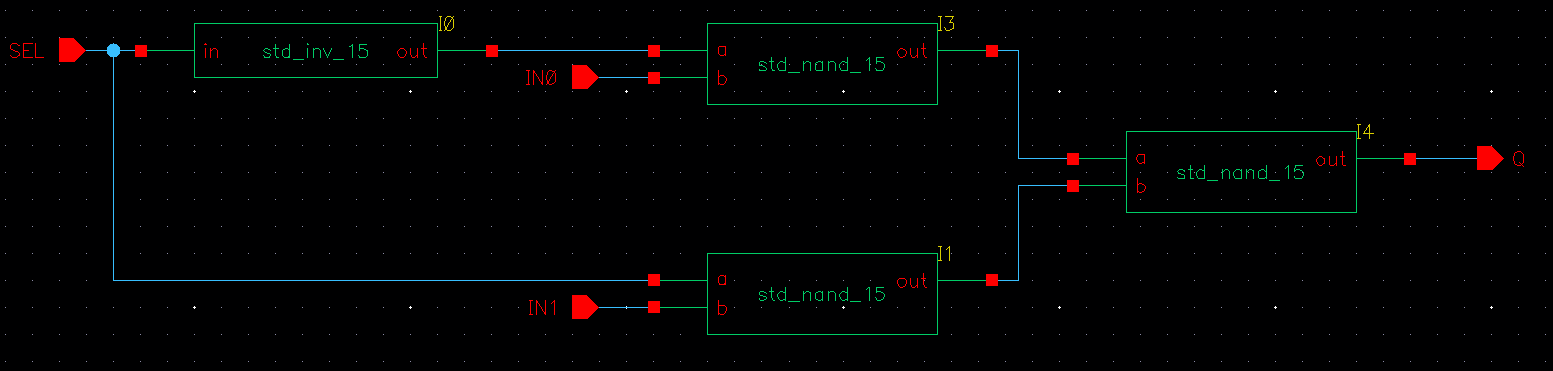
\includegraphics[width=5in]{figures/schem.png}
  \caption{Transistor-level Mux Schematic}\label{fig:schem}
\end{figure}
Figure~\ref{fig:sim} shows the simulation schematic with the source and load. 
Three different pulses are used so we can measure the propagation delay of the select signal
given different sets of input signals. All the pulses have an amplitude of 1.2V, a rise time of
10ps, and a fall time of 10ps.
While the inputs have a pulse width of 3ns and a period of 6ns, the select signal has a pulse width of 1ns and a
period of 2ns. The only signal with a delay is in1 with a value of 3ns, which allows us to get the values we need
on the table.
A 10fF capacitor was tied to the output to get it closer to a realistic model where the output of the
multiplexer would have some capacitance.
\begin{figure}[!htb]
  \centering
  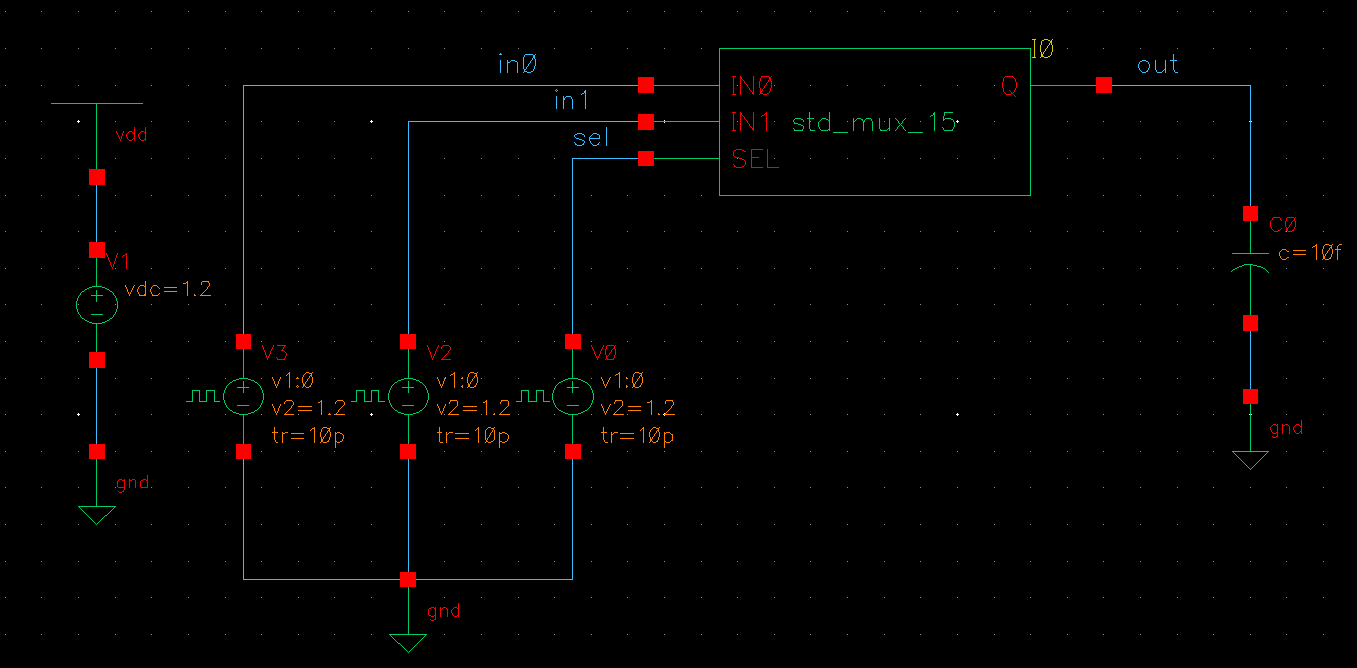
\includegraphics[width=5in]{figures/sim.png}
  \caption{Mux Simulation Schematic}\label{fig:sim}
\end{figure}
The transient analysis is shown in Figure~\ref{fig:transient}. Using the transient analysis graph
rise time of 108.52ps and a fall time of 52.49ps were easily found. 
The values for the propagation delays are listed in Table~\ref{table:results}.
\begin{figure}[!htb]
  \centering
  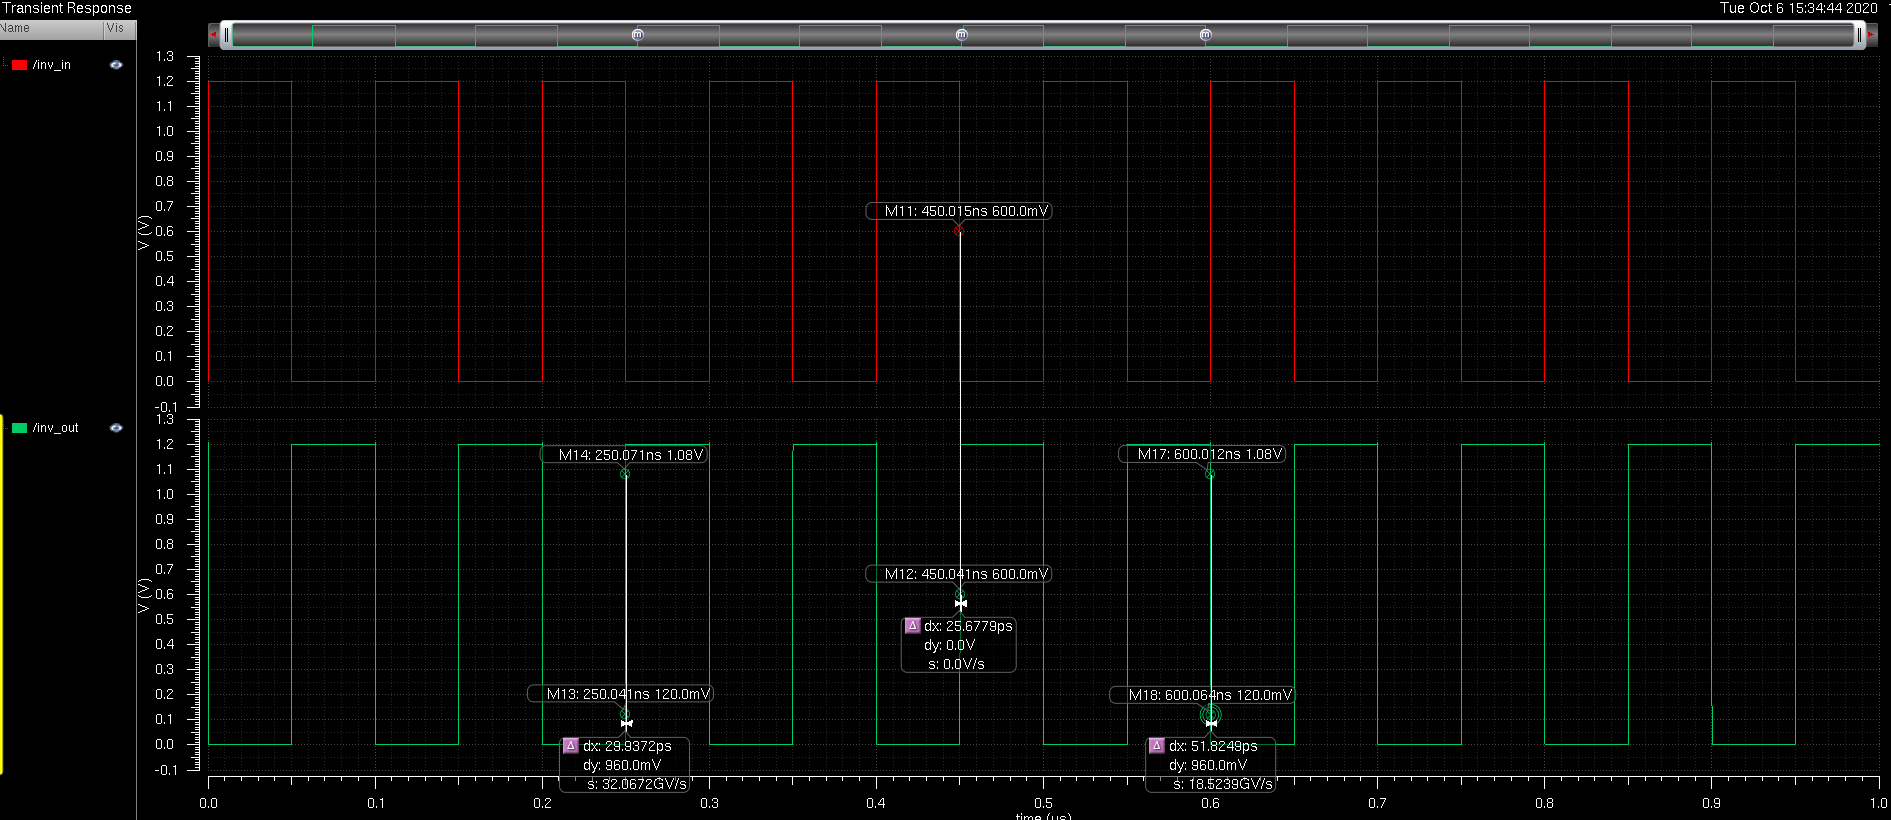
\includegraphics[width=5in]{figures/transient.png}
  \caption{Mux Transient Analysis}\label{fig:transient}
\end{figure}
\begin{table}[!htb]
  \centering
  \caption{Propagation Delay of Select}\label{table:results}
  \begin{tabular}{ |l|l|l|l|l| }
    \hline
    IN0 & IN1 & SEL & Q & Delay(ps) \\
    \hline
    0 & 1 & 0 & 0 & 49.26 \\
    0 & 1 & 1 & 1 & 89.77 \\
    1 & 0 & 0 & 1 & 91.24 \\
    1 & 0 & 1 & 0 & 54.20 \\
    \hline
  \end{tabular}
\end{table}
\subsection{Layout Design}
After the multiplexer's schematic was finished, layout was done. The layout was done using
pitch matching and using the previous layouts that were created for the symmtric gates.
After the gates' layouts were place metal was placed between the designs and the pins were
placed. A second metal was also used to route parts that are supposed to be tied together, but are
on opposite sides of the design. The layout is shown in Figure~\ref{fig:layout}.
\begin{figure}[!htb]
  \centering
  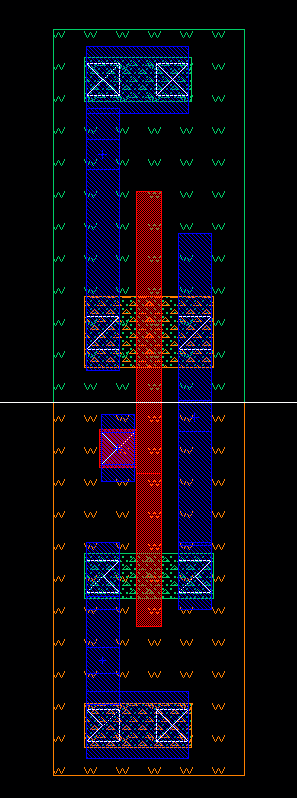
\includegraphics[width=5in]{figures/layout.png}
  \caption{Mux Layout}\label{fig:layout}
\end{figure}
Lastly, design rule checking(DRC) is used to make sure that no design rules are being violated and
everything is fixed very painstakingly. The results for the design rule checking are shown in
Figure~\ref{fig:drc}. After that layout versus schematic(LVS) was used to make sure the layout matches
the design modeled with the schematic and is shown in Figure~\ref{fig:lvs}.
\begin{figure}[!htb]
  \centering
  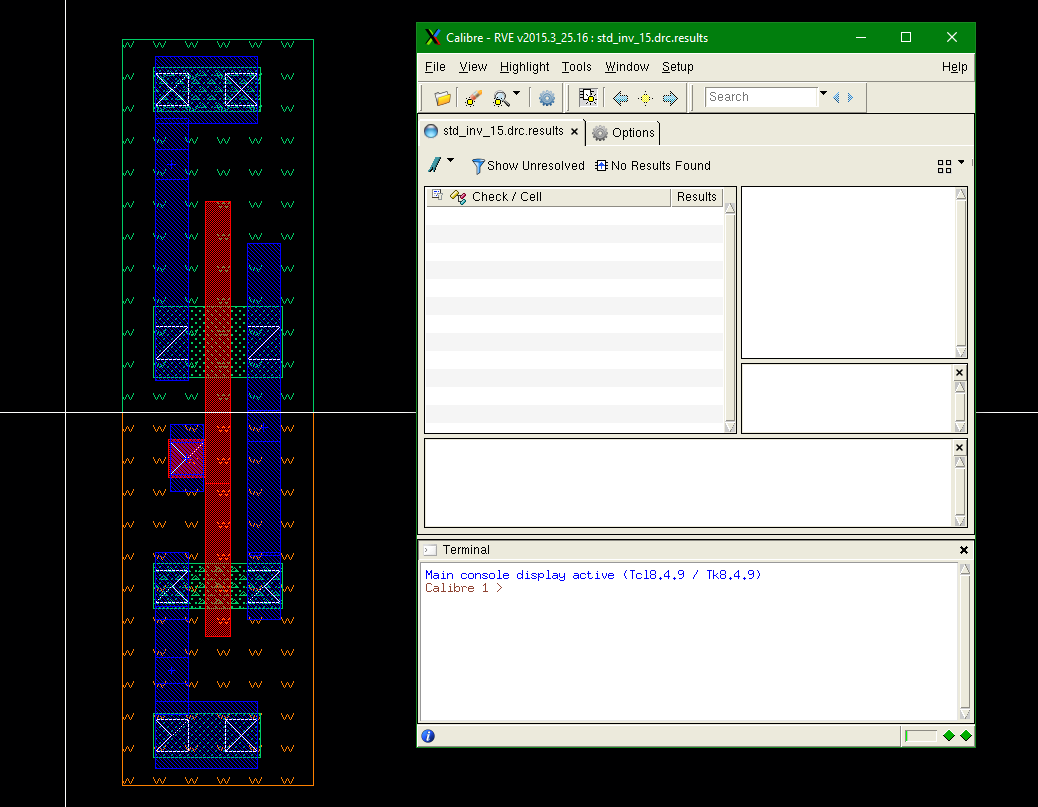
\includegraphics[width=3.5in]{figures/drc.png}
  \caption{DRC Results}\label{fig:drc}
\end{figure}
\begin{figure}[!htb]
  \centering
  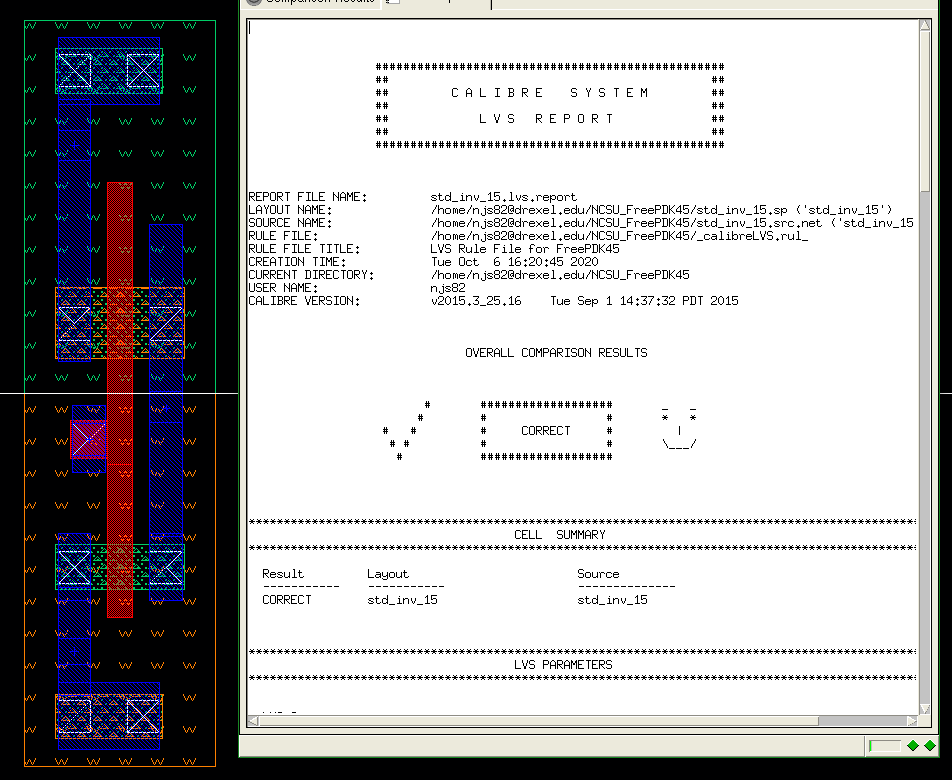
\includegraphics[width=3.5in]{figures/lvs.png}
  \caption{LVS Results}\label{fig:lvs}
\end{figure}
\clearpage
\section{Conclusion}
The lab was a great way to cement everything that was learned previously and get even further experience
creating a layout with previously designed gates. Pitch matching saves a lot of time in the long run and
allows heavy design reuse. It also helped in tracking down any issues as the designs of the gates have
been verified, so if there was anything wrong, it was easy to figure out that it was in the interconnection
of the separate gates. This lab allowed us to get insight into one of the most important tools in any
digital designers toolbox, the multiplexer.
\end{document}
%%% Local Variables:
%%% mode: latex
%%% TeX-master: t
%%% End:
